\ifx \allfiles \undefined		%编译PPT时注释该行
\documentclass{ctexart}				%编译PPT时注释该行
\usepackage{ifthen}
%\usepackage[a3paper,landscape,showframe,margin=1.25in]{geometry}
%\usepackage[a3paper,landscape,margin=1.1in]{geometry}
\usepackage[a3paper,landscape,top=1.25in,bottom=0.8in,left=1in,right=1in]{geometry}
\usepackage{tikz,units}
\usepackage{circuitikz}
\usepackage{subfig}
\usetikzlibrary{backgrounds,circuits.ee.IEC.relay}
\usetikzlibrary{positioning}
\usepackage{tikzsymbols}
\usepackage{pgffor}
\usetikzlibrary {math}
\usepackage{lastpage}
\usepackage{fancyhdr}
\pagestyle{fancy}
\fancyhf{}
\fancyhead[ER,OL]{\heiti \zihao{-5} 热工专业图纸}
\fancyhead[OR,EL]{\heiti \zihao{-5} \leftmark}
\fancyfoot[CE,CO]{热工专业图纸~第~\thepage~页(共 \pageref{LastPage} 页)}
\renewcommand{\headrulewidth}{0.4pt}
\renewcommand{\footrulewidth}{0.4pt}
\tikzset{
box/.style={rectangle,minimum height=17pt,minimum width=20pt,text=red}
}
\tikzset{
boxA/.style={rectangle,minimum height=17pt,minimum width=20pt,draw=black}
}
\tikzset{
boxB/.style={rectangle,minimum height=17pt,minimum width=30pt,draw=black}
}
\tikzset{
boxC/.style={rectangle,minimum height=17pt,minimum width=120pt,draw=black}
}
\tikzset{
boxD/.style={minimum width=140pt,above left}
}

\lhead{热工专业图纸}
\rhead{给煤机插板门电气原理图}
\cfoot{热工专业图纸~第~\thepage~页 (共 \pageref{LastPage} 页)}
\begin{document}
		\else						%编译PPT时注释该行
		\chapter{给煤机插板门电气原理图}	%编译PPT时注释该行
		\newpage
		\fi						%编译PPT时注释该行
\begin{center}
{\huge 给煤机插板门电气原理图}
\end{center}
\begin{center}

	\begin{figure}[h]
\subfloat[动力回路]{
\label{fig:improved_subfig_a}
		\begin{minipage}{300pt}
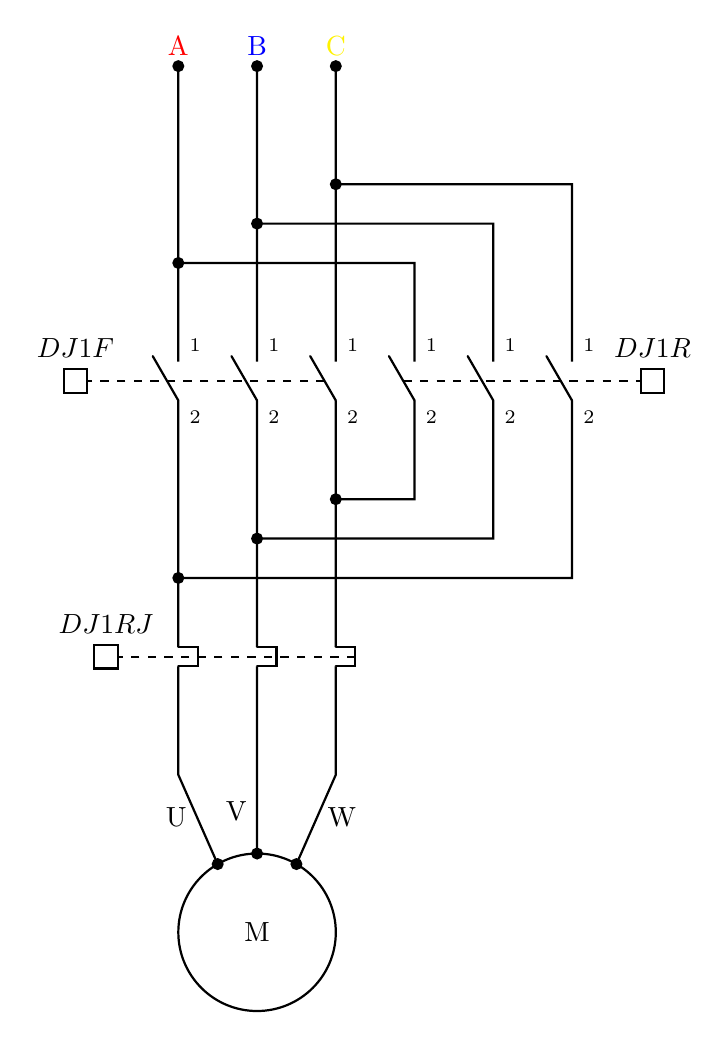
\begin{tikzpicture}[circuit ee IEC relay,thick,scale=1]
%d动力回路
\node (M) at (1,0) {M};%绝对坐标
\coordinate (V1) at (1,2);
\coordinate[right=1 of V1] (W1);
\coordinate[left=1 of V1] (U1);
\draw (M) circle (1);

\draw (M) ++(120:1) node [contact,name=U]{};
\draw (M) ++(90:1) node [contact,name=V]{};
\draw (M) ++(60:1) node [contact,name=W]{};

\draw (V) -- node[left] {V} (V1) -- ++(0,1)
to [thermic sensor] ++(0,1) -- ++(0,1)
node [contact,name=V2]{} -- ++(0,1.5)
to [make contact={term=1,term'=2}] ++(0,1) -- ++(0,1.5)
node [contact,name=V3]{} -- ++(0,2)
node [contact,name=V4]{};
\node[above,blue] at(V4) {B};

\draw (U) -- node[left] {U} (U1) -- ++(0,1)
to [thermic sensor] ++(0,1) -- ++(0,0.5)
node [contact,name=U2]{} -- ++(0,2)
to [make contact={term=1,term'=2}] ++(0,1) -- ++(0,1)
node [contact,name=U3]{} -- ++(0,2.5)
node [contact,name=U4]{};
\node[above,red] at(U4) {A};

\draw (W) -- node[right] {W} (W1) -- ++(0,1)
to [thermic sensor={name=FR}] ++(0,1) -- ++(0,1.5)
node [contact,name=W2]{} -- ++(0,1)
to [make contact={name=KM1,term=1,term'=2}] ++(0,1) -- ++(0,2)
node [contact,name=W3]{} -- ++(0,1.5)
node [contact,name=W4]{};
\node[above,yellow] at(W4) {C};

\draw (V2) -- ++(3,0) -- ++(0,1.5) to [make contact={term=1,term'=2}] ++(0,1) -- ++(0,1.5) -- (V3);

\draw (U2) -- ++(5,0) -- ++(0,2) to [make contact={term=1,term'=2}] ++(0,1) -- ++(0,2) -- (W3);

\draw (W2) -- ++(1,0) -- ++(0,1) to [make contact={name=KM2,term=1,term'=2}] ++(0,1) -- ++(0,1) -- (U3);

\draw[dashed](KM1.mid) -- ++(-3,0) node[left,draw,solid,minimum size=3mm,label={[above]:$DJ1F$}]{};

\draw[dashed](KM2.mid) -- ++(3,0) node[right,draw,solid,minimum size=3mm,label={[above]:$DJ1R$}]{};

\draw[dashed](FR.mid) -- ++(-3,0) node[left,draw,solid,minimum size=3mm,label={[above]:$DJ1RJ$}]{};

	\end{tikzpicture}
		\end{minipage}
}
\subfloat[控制回路]{
\label{fig:improved_subfig_b}
		\begin{minipage}{600pt}
\begin{tikzpicture}[circuit ee IEC relay,thick,
	x=12\tikzcircuitssizeunit,
	y=6\tikzcircuitssizeunit,
	every term/.style={gray,font=\scriptsize},
	every term'/.style=every term,
	every term''/.style=every term]
		
			\draw (0,0) node [contact,name=A]{} -- ++(1,0) node [shape=coordinate](A1){}  -- ++(1,0) node [contact,name=B1]{}
				-- ++(1,0)node [shape=coordinate](C1){}  -- ++(0.5,0)node [contact,name=D]{}-- ++(0.5,0)node [contact,name=D1]{} -- ++(0.5,0) node [contact,name=E]{} -- ++(0.5,0) node [contact,name=E1]{} -- ++(0.5,0) node [contact,name=F]{} -- ++(0.5,0) node [contact,name=F1]{} -- ++(1,0) node [shape=coordinate](G1){} ;
		\draw (A) -- ++(0,1)
		to [bulb={info=H4}] ++(0,1) -- ++(0,7)
		node [contact,name=A8]{};
		\draw (B1)
		to [change over contact={name=sw1,info=K7.3,term=7,term'=11,term''=3}] ++(0,1) coordinate(n1) -- ++(0,1)
		node [contact,name=B2]{}
		to [break contact={thermal switch={info=$KR1$}}] ++(0,1)
		node [contact,name=B3]{};
		\draw (sw1.output 1) -- (sw1.output 1 |- n1)
		to [break contact={push button={info=$SB1$}}] ++(0,0.5) -- ++(0,0.5) -- (B2);
		\draw (B3) -- ++(-1,0)
		to [relay coil={info=$KM1$,term=A1,term'=A2}] ++(0,1)
		node [contact,name=A4]{}
		to [change over contact={name=sw2,info=K7.1,term=5,term'=9,term''=1}] ++(0,1) coordinate(n2)
		to [make contact={info={[right=0.3cm]:远开}}] ++(0,0.5) -- ++(0,0.5)
		node [contact,name=A5]{}
		to [break contact={info=$KM2$}] ++(0,1)
		node [contact,name=A6]{}
		to [break contact={position switch={info=$LS01$}}] ++(0,1)
		to [break contact={position switch={info=$TS01$}}] ++(0,1)
		node [contact,name=A7]{};

		\draw (A4) -- ++(0.5,0) -- ++(0,1)
		to [make contact={info={[right=0.3cm]:$KM1$}}] ++(0,0.5) -- ++(0,0.5) -- (A5);
		\draw (sw2.output 1) -- (sw2.output 1 |- n2)
		to [make contact={push button={info=$SB3$}}] ++(0,0.5) -- ++(0,0.5) -- (A5);
		\draw (B3) -- ++(1,0)
		to [relay coil={info=$KM1$,term=A1,term'=A2}] ++(0,1)
		node [contact,name=C4]{}
		to [change over contact={name=sw3,info=K7.2,term=6,term'=10,term''=2}] ++(0,1) coordinate(n3)
		to [make contact={info={[right=0.3cm]:远关}}] ++(0,0.5) -- ++(0,0.5)
		node [contact,name=C5]{}
		to [break contact={info=$KM2$}] ++(0,1)
		node [contact,name=C6]{}
		to [break contact={position switch={info=$LS01$}}] ++(0,1)
		to [break contact={position switch={info=$TS01$}}] ++(0,1)
		node [contact,name=C7]{};
		\draw (C4) -- ++(0.5,0)
		to [make contact={info={[right=0.3cm]:$KM2$}}] ++(0,2) -- (C5);
		\draw (sw3.output 1) -- (sw3.output 1 |- n3)
		to [make contact={push button={info=$SB3$}}] ++(0,0.5) -- ++(0,0.5) -- (C5);
		\draw (D1) -- ++(0,1)
		to [bulb={info=H5}] ++(0,1)
		node [contact,name=D2]{}
		-- ++(0,5) node [contact,name=D3]{}
		to [make contact={position switch={info=$LSO1$}}] ++(0,2)
		node [contact,name=D4]{};
		\draw (D)
		to [relay coil={info=$K1$,term=13,term'=14}] ++(0,1) -- ++(0,1) -- (D2);

		\draw (E1) -- ++(0,1)
		to [bulb={info=H4}] ++(0,1)
		node [contact,name=E2]{}
		-- ++(0,5) node [contact,name=E3]{}
		to [make contact={position switch={info=$LSC1$}}] ++(0,2)
		node [contact,name=E4]{};
		\draw (E)
		to [relay coil={info=$K2$,term=13,term'=14}] ++(0,1) -- ++(0,1) -- (E2);

		\draw (F1) -- ++(0,1)
		to [bulb={info=H2}] ++(0,1)
		node [contact,name=F3]{} -- ++(0,3) 
		node [contact,name=F4]{} -- ++(0,2) 
		node [contact,name=F5]{}
		to [make contact={position switch={info=$TSC1$}}] ++(0,2)
		node [contact,name=F6]{};
		\draw (F)
		to [relay coil={info=$K3$,term=13,term'=14}] ++(0,1) -- ++(0,1) -- (F3);
	\draw (F5) -- ++(-0.5,0)
		to [make contact={position switch={info=$TSO1$}}] ++(0,2)
		node [contact,name=F]{};
		;
	\draw (F4) -- ++(0.5,0)
		to [make contact={thermal switch={info={[above=0.3cm]:$KR1$}}}] ++(0,1)
		-- ++(0,3) node [contact,name=F7]{};
		\draw (G1) -- ++(0,2)
		to [relay coil={info=$K7$,term=13,term'=14}] ++(0,1) -- ++(0,1)
		to [make contact={turn switch={info=$SB3$}}] ++(0,1)
		-- ++(0,4) node [shape=coordinate](G2){} ;
		\draw (G2) -- (A8)
		to [fuse={info={$\unit[2]{A}$}}] ++(-0.5,0)
		node[below]{L};
	\draw (A) -- ++(-0.5,0)
		node[above]{N};
	\end{tikzpicture}

		\end{minipage}
}
\caption{给煤机插板门电气回路图}
\label{fig:improved_subfig}
	\end{figure}
\end{center}
		\ifx \allfiles \undefined
\end{document}

\fi
